\documentclass[14pt]{article}

\usepackage[utf8]{inputenc}
\usepackage[russian]{babel}
\usepackage{amsmath,amssymb}

\usepackage{geometry}
\geometry{
	a4paper,
	total={170mm,257mm},
	left=20mm,
	top=10mm,
	}

\usepackage{graphicx}
\usepackage{tabularx, ragged2e, booktabs, caption}

\newcommand{\lb}{\left(}
\newcommand{\rb}{\right)}

\newcommand{\mH}{\mathcal{H}}

\newcolumntype{C}[1]{>{\Centering}m{#1}}
\renewcommand\tabularxcolumn[1]{C{#1}}

\makeatletter
\providecommand\barcirc{\mathpalette\@barred\circ}%
\def\@barred#1#2{\ooalign{\hfil$#1-$\hfil\cr\hfil$#1#2$\hfil\cr}}%
\newcommand\stst{^{\protect\barcirc}}%
\makeatother

\begin{document}

Рассмотрим гамильтониан системы $Ar-CO_2$ в молекулярно-фиксированной системе координат:
\begin{gather}
\mH_{mol} = \frac{1}{2 \mu_2} p_R^2 + \lb \frac{1}{2 \mu_2 R^2} + \frac{1}{2 \mu_1 l^2} \rb p_\theta^2 - \frac{1}{\mu_2 R^2} p_\theta J_y + \frac{1}{2 \mu_2 R^2} J_y^2 + \frac{1}{2 \mu_2 R^2} J_x^2 + \frac{1}{2 \sin^2 \theta} \lb \frac{\cos^2 \theta}{\mu_2 R^2} + \frac{1}{\mu_1 l^2} \rb J_z^2 + \notag \\
+ \frac{\ctg \theta}{\mu_2 R^2} J_x J_z + U(R, \theta) \notag
\end{gather}

Выделяя полные квадраты, приходим к следующему выражению:
\begin{gather}
	\mH_{mol} = \frac{p_R^2}{2 \mu_2} + \frac{p_\theta^2}{2 \mu_1 l^2} + \frac{1}{2 \mu_2 R^2} \lb p_\theta - J_y \rb^2 + \frac{1}{2 \mu_2 R^2} \lb J_x + J_z \ctg \theta \rb^2 + \frac{J_z^2}{2 \mu_1 l^2 \sin^2 \theta} + U(R, \theta) \notag
\end{gather}

Произведем следующую линейную замену координат, позволяющую представить отношение гамильтониана к $kT$ в предельно простой форме ($p_R, p_\theta, J_x, J_y, J_z \rightarrow x_1, x_2, x_3, x_4, x_5$, причем $R, \theta$ считаем постоянными при осуществлении замены):
\begin{gather}
	\left\{
	\begin{aligned}
	x_1^2 &= \frac{p_R^2}{2 \mu_2 kT} \\
	x_2^2 &= \frac{p_\theta^2}{2 \mu_1 l^2 kT} \\
	x_3^2 &= \frac{ \lb p_\theta - J_y \rb^2}{2 \mu_2 R^2 k T} \\
	x_4^2 &= \frac{ \lb J_x + J_z \ctg \theta \rb^2}{2 \mu_2 R^2 k T} \\
	x_5^2 &= \frac{J_z^2}{2 \mu_1 l^2 \sin^2 \theta kT}
	\end{aligned}
	\right. \quad \implies \quad 
	\left\{
	\begin{aligned}
	dx_1 &= \frac{dp_R}{\sqrt{ 2 \mu_2 k T}} \\
	dx_2 &= \frac{dp_\theta}{\sqrt{2 \mu_1 l^2 k T}} \\
	dx_3 &= \frac{dp_\theta - dJ_y}{\sqrt{2 \mu_2 R^2 k T}} \\
	dx_4 &= \frac{dJ_x + \ctg \theta dJ_z}{ \sqrt{2 \mu_2 R^2 k T}} \\
	dx_5 &= \frac{dJ_z}{\sqrt{2 \mu_1 l^2 \sin^2 \theta k T}}
	\end{aligned}
	\right. \quad \implies \quad
	\left\{
	\begin{aligned}
		dp_R &= \sqrt{2 \mu_2 k T} dx_1 \\
		dp_\theta &= \sqrt{2 \mu_1 l^2 kT} dx_2 \\
		dJ_y &= \sqrt{2 \mu_1 l^2 kT} dx_2 - \sqrt{2 \mu_2 R^2 kT} dx_3 \\
		dJ_x &= \sqrt{2 \mu_2 R^2 kT} dx_4 - \sqrt{2 \mu_1 l^2 \cos^2 \theta kT} dx_5 \\
		dJ_z &= \sqrt{2 \mu_1 l^2 \sin^2 \theta kT} dx_5
	\end{aligned}
	\right.
	\notag
\end{gather}

Разобъем фазовый интеграл на две части (основываясь на теореме Фубини?) -- на интеграл по $R, \theta$ и на интеграл по всему остальному, также как делается в статье Андрея Алексеевича (причем внутренний интеграл берется при фиксированных значениях $R, \theta$):
\begin{gather}
	\frac{1}{h^5} \int_{H < 0} \exp \lb -\frac{H_{mol}}{kT} \rb dR dp_R d\theta dp_\theta dJ_x dJ_y dJ_z = \frac{1}{h^5} \int \int dR d\theta \int \exp \lb -\frac{H_{mol}}{kT} \rb dp_R dp_\theta dJ_x dJ_y dJ_z \notag	
\end{gather}
Применим приготовленную замену:
\begin{gather}
	\frac{1}{h^5} \int \int dR d\theta \int \exp \lb -\frac{H_{mol}}{kT} \rb dp_R dp_\theta dJ_x dJ_y dJ_z = \frac{1}{h^5} \int \int [Jac \, ] \exp \lb -\frac{U}{kT} \rb dR d\theta \times \notag \\ \times \int_{x_1^2 + \dots + x_5^2 + \frac{U}{kT} < 0} \exp \lb - x_1^2 - \dots - x_5^2 \rb dx_1 \dots dx_5, \notag 
\end{gather}

где $[Jac \,]$ представляет собой следующее выражение (основываясь на представлении о том, что конструкцию $dx_1 dx_2 dx_3 dx_4 dx_5$ \textit{можно воспринимать} как дифференциальную форму $dx_1 \wedge dx_2 \wedge dx_3 \wedge dx_4 \wedge dx_5$, зануляю интегралы, которые содержат пару одинаковых $dx_i$; короче говоря, пара одинаковых $dx_i$ будет означать вырожденность элемента объема, что автоматически зануляет интеграл):
\begin{gather}
	[Jac\,] = \frac{\partial [p_R, p_\theta, J_x, J_y, J_z]}{\partial [x_1, x_2, x_3, x_4, x_5]} = \sqrt{2 \mu_2 k T} \sqrt{2 \mu_1 l^2 k T} \sqrt{2 \mu_2 R^2 kT} \sqrt{2 \mu_2 R^2 kT} \sqrt{2 \mu_1 l^2 \sin^2 \theta kT} = \notag \\
	= kT (2 \mu_2 kT)^\frac{3}{2} 2\mu_1 l^2 R^2 \sin \theta \notag
\end{gather}

Применим формулу $(A13)$ к интегралу по многомерному шару:
\begin{gather}
	\int_{x_1^2 + \dots x_5^2 + \frac{U}{kT} < 0} \exp \lb -x_1^2 - \dots -x_5^2 \rb dx_1 \dots dx_5 = \pi^\frac{5}{2} \frac{\gamma \lb \frac{5}{2}, - \frac{U}{kT} \rb}{\Gamma \lb \frac{5}{2} \rb} \notag
\end{gather}

Итак, фазовый интеграл сводится к следующему интегралу по двумерной области, где $U(R, \theta) < 0$ (не имеет смысла интегрировать по $R, \theta$ вне нее,т.к. радиус шара, по которому берется внутренний интеграл, положителен, только в случае отрицательного значения потенциала):
\begin{gather}
	\frac{1}{h^5} \int_{H < 0} \exp \lb -\frac{U}{kT} \rb dp_R dp_\theta dJ_x dJ_y dJ_z = \lb \frac{2 \pi \mu_2 k T}{h^2} \rb^{\frac{3}{2}} \frac{2 \mu_1 l^2 \pi k T}{h^2} \int \int_{U < 0} \exp \lb -\frac{U}{kT}\rb \frac{\gamma \lb \frac{5}{2}, - \frac{U}{kT} \rb}{\Gamma \lb \frac{5}{2} \rb} R^2 \sin \theta dR d\theta \notag 
\end{gather}

Преобразуем второй множитель к виду вращательной статсуммы $CO_2$:
\begin{gather}
	l = 2 r_{C-O}, \mu_1 = \frac{m_O}{2} \notag \\
	Q_{rot} = \frac{8 \pi^2 k T}{h^2} m_O r_{C-O}^2 = \frac{4 \pi^2 k T}{h^2} \mu_1 l^2 \notag \\
	\frac{2 \mu_1 l^2 \pi k T}{h^2} =  \frac{1}{2 \pi} Q_{rot} \notag \\
	Q_{CO_2} = \frac{1}{\sigma} Q_{tr} Q_{rot} = \frac{1}{2} Q_{tr} Q_{rot} \notag
\end{gather}

Итак, статсумма связанного димера $Ar-CO_2$ преобразуется к следующему виду:
\begin{gather}
	Q^{bound}_{pair} = \lb \frac{2 \pi M k T}{h^2} \rb^\frac{3}{2} V \frac{1}{h^5} \int_{H < 0} \exp \lb - \frac{H_{mol}}{kT} \rb dR dp_R d\theta dp_\theta dJ_x dJ_y dJ_z d \Phi d\Theta d\Psi = \notag \\ 
	= 4 \pi Q_{Ar} Q_{CO_2} \int \int_{U < 0} \exp \lb -\frac{U}{kT}\rb \frac{\gamma \lb \frac{5}{2}, - \frac{U}{kT} \rb}{\Gamma \lb \frac{5}{2} \rb} R^2 \sin \theta dR d\theta \notag
\end{gather}

Приходим к следующему выражению для константы равновесия:
\begin{gather}
	K_p = \frac{4 \pi N_0}{R T} \int \int_{U < 0} \exp \lb -\frac{U}{kT}\rb \frac{\gamma \lb \frac{5}{2}, - \frac{U}{kT} \rb}{\Gamma \lb \frac{5}{2} \rb} R^2 \sin \theta dR d\theta \notag 
\end{gather}

\newpage

Сравним значения получаемые при интегрировании гамильтониана по области фазового пространства с интегралом по потенциальной области следующим образом:
\begin{gather}
	(1): \int \int_{U < 0} \exp \lb -\frac{U}{kT} \rb \frac{\gamma \lb \frac{5}{2}, -\frac{U}{kT} \rb}{\Gamma \lb \frac{5}{2} \rb } R^2 \sin \theta dR d \theta \notag \\
	(2): \frac{1}{\lb 2 \mu_2 kT \rb^{\frac{3}{2}}} \frac{1}{2 \mu_1 l^2 kT} \int_{H < 0} \exp \lb - \frac{H_{mol}}{kT} \rb dR dp_R d\theta dp_\theta dJ_x dJ_y dJ_z \notag
\end{gather}

\begin{center}
\begin{tabular}{ccc}
	\hline
	Температура & $(1)$ & $(2)$ \\
	\hline
	100K & 521.833 & 521.392 \\
	150K & 151.053 & 151.121 \\
	200K & 66.442 &  66.376 \\
	250K & 35.884 & 35.802 \\
	\hline
\end{tabular} 
\end{center}

\vspace{0.3cm}
С точностью до погрешности Монте-Карло формулы $(2)$ и $(3)$ дают одинаковый результат. (Интеграл в $(3)$ имеет порядок примерно $1 \cdot 10^8$, так что погрешности там могут быть достаточно существенными.)

(При построении графика предполагаю, что потерял $2$ку в предынтегральном множителе, то есть следующий его вид: $\frac{2 \pi N_0}{RT}$.) 

Температурная зависимость константы равновесия в обратных атмосферах; Simple formula -- $(1)$, General formula -- $(2)$ = $(3)$.

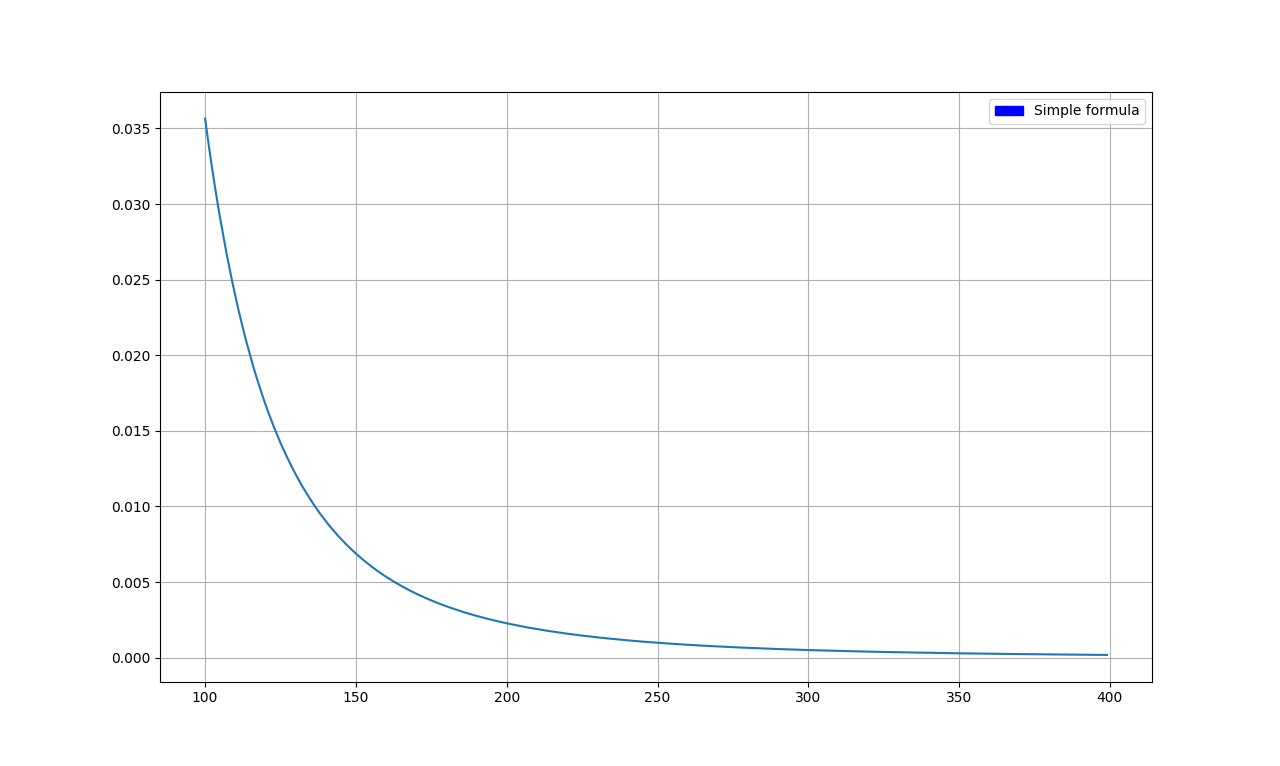
\includegraphics[scale=0.5]{plot.png}

\newpage

\begin{gather}
	\frac{1}{\lb 2 \mu_2 k T \rb^{\frac{3}{2}}} = V \frac{\pi^{\frac{3}{2}}}{h^3} \frac{Q_{complex}^{tr}}{Q_{CO_2}^{tr} Q_{Ar}^{tr}} \notag \\
	\frac{1}{2 \mu_1 l^2 k T} = \frac{2 \pi^2}{h^2} \frac{1}{Q_{CO_2}^{rot}} \notag \\
	\frac{1}{\lb 2 \mu_2 k T \rb^{\frac{3}{2}}} \times \frac{1}{2 \mu_1 l^2 k T} = \frac{2 \pi^{\frac{7}{2}}}{h^5} V \frac{Q_{complex}^{tr}}{Q_{CO_2}^{tr} Q_{CO_2}^{rot} Q_{Ar}^{tr}} = \frac{4 \pi^{\frac{7}{2}}}{h^5} V \frac{Q_{complex}^{tr}}{Q_{CO_2} Q_{Ar}} \notag \\
	K_p = \frac{2 \pi N_0}{RT} \int \int_{U < 0} \frac{\gamma \lb \frac{5}{2} , - \frac{U}{kT} \rb }{\Gamma \lb \frac{5}{2} \rb} \exp \lb - \frac{U}{kT} \rb R^2 \sin \theta dR d\theta \notag \\
	K_p = \frac{2 \pi N_0}{RT}  \frac{1}{\lb 2 \mu_2 k T \rb^{\frac{3}{2}}} \frac{1}{2 \mu_1 l^2 k T} \times \int_{H < 0} \exp \lb - \frac{H}{kT} \rb dR dp_R d\theta dp_\theta dJ_x dJ_y dJ_z = \notag \\
	= \frac{N_0}{p} \frac{Q_{complex}^{tr}}{Q_{CO_2} Q_{Ar}} \pi^\frac{5}{2} \frac{1}{h^5} \int_{H < 0} \exp \lb - \frac{H}{kT} \rb dR dp_R d\theta dp_\theta d\Theta d\Phi d\Psi dp_\Theta dp_\Psi dp_\Theta \notag
\end{gather}

\newpage

Рассмотрим $n$-мерную гиперсферу (гипершар). Исходя из соображений размерности (dimensional analysis) объем гиперсферы должен быть пропорционален $n$-ой степени $R$:
\begin{gather}
	V_n (R) = \int \dots \int_{x_1^2 + \dots x_n^2 \leq R^2} dx_1 \dots dx_n = C_n R^n \notag
\end{gather}

Объем сферы $V_n(R)$ может быть получен путем интегрирования площади сферических слоев $S_{n-1}(R)$ по радиусу сферы:
\begin{gather}
	V_n(R) = \int_{0}^{R} S_{n-1}(r) dr \notag \\
	S_{n-1}(R) = \frac{d V_n(R)}{dR} = nC_n R^{n-1} \notag 
\end{gather}

Таким образом, очевидно, что интеграл по гиперсферическим координатам дает $nC_n$:
\begin{gather}
	\int \dots \int_{x_1^2 + \dots x_n^2 \leq R^2} dx_1 \dots dx_n = n C_n \int_{0}^{R} r^{n-1} dr = \int \dots \int d \Omega_{n-1} \int_{0}^{R} r^{n-1} dr \notag \\
	\int \dots \int d \Omega_{n-1} = n C_n \notag
\end{gather}

Для того, чтобы получить численное выражение для $C_n$ рассмотрим интеграл функции $f(x_1, \dots x_n) = \exp \lb -x_1^2 - \dots x_n^2 \rb$ по всему объему $n$-мерного пространства. Сразу же осуществим переход к гиперсферическим координатам, учитывая вышеизложенные факты:
\begin{gather}
	\int_{-\infty}^{\infty} \dots \int_{-\infty}^{\infty} \exp \lb -x_1^2 - \dots -x_n^2 \rb dx_1 \dots dx_n = \int_{0}^{\infty} \exp \lb -r^2 \rb r^{n-1} dr \int d \Omega_{n-1}  = n C_n \int_{0}^{R} r^{n-1} \exp \lb -r^2 \rb dr= \notag \\
	= \frac{1}{2} \Gamma \lb \frac{n}{2} \rb n C_n \notag
\end{gather}

Одновременно, многомерный интеграл представим в виде произведения одномерных интегралов Пуассона:
\begin{gather}
	\int_{-\infty}^{\infty} \dots \int_{-\infty}^{\infty} \exp \lb -x_1^2 - \dots - x_n^2 \rb d x_1 \dots dx_n = \left[ \int_{-\infty}^{\infty} \exp \lb -x_1^2 \rb dx_1 \right]^n  = \pi^\frac{n}{2} \notag 
\end{gather}

Итак, получаем следующее выражение для $C_n$:
\begin{gather}
	C_n = \frac{\pi^\frac{n}{2}}{\frac{n}{2} \Gamma \lb \frac{n}{2} \rb} \notag
\end{gather}

Рассмотрим интеграл все той же экспоненты, но уже по объему $n$-мерной гиперсферы. Как и раньше, перейдем к гиперсферическим координатам:
\begin{gather}
	\int \dots \int_{x_1^2 + \dots + x_n^2 \leq R^2} \exp \lb -x_1^2 - \dots - x_n^2 \rb dx_1 \dots dx_n = \int_{0}^{R} r^{n-1} \exp \lb -r^2 \rb dr \int d \Omega_{n-1} = \notag \\
	= \frac{2 \pi^{\frac{n}{2}}}{\Gamma \lb \frac{n}{2} \rb} \int_{0}^{R} r^{n-1} \exp \lb -r^2 \rb dr = \left[ t = r^2 \right] = \frac{\pi^{\frac{n}{2}}}{\Gamma \lb \frac{n}{2} \rb} \int_{0}^{R^2} t^{\frac{n}{2} - 1} \exp \lb -t \rb dt = \frac{\pi^{\frac{n}{2}}}{\Gamma \lb \frac{n}{2} \rb} \gamma \lb \frac{n}{2}, R^2 \rb \notag
\end{gather}

\newpage

\section*{Расчет константы равновесия в каноническом ансамбле}

Канонический ансамбль -- модель термодинамической системы, окруженной полупроницаемой (пропускает энергию, но не материю == diathermal) жесткой стенкой, погруженной в тепловой резервуар постоянной температуры. Тепловой резервуар обеспечивает постоянство температуры внутри рассматриваемой системы независимо от того в какую сторону протекает тепловой поток между ними. Таким образом, канонический ансамбль -- также называемый $NVT$-ансамблем -- состоит из $N$ частиц, находящихся в фиксированном объеме $V$ при фиксированной температуре $T$.  Рассматривая совокупность резервуара и погруженной в него исследуемой системы как микроканонической системы, получают каноническое распределение (распределение Гиббса) -- вероятность нахождения системы в состоянии с энергией $E_n$:
\begin{gather}
	\omega_n = A \times \exp \lb - \frac{E_n}{kT} \rb \quad \Leftrightarrow \quad \rho \lb p, q \rb = A \times \exp \lb - \frac{E \lb p, q \rb}{kT} \rb \notag
\end{gather}
Энтропия может быть выражена как среднее значение функции распределения:
\begin{gather}
	S = - \langle \ln \omega_n \rangle \notag \\
	S = - \ln A + \frac{1}{T} \langle E_n \rangle = - \ln A + \frac{\overline{E}}{kT} \notag \\
	\ln A = \frac{\overline{E} - TS}{kT} = \frac{F}{kT} \notag 
\end{gather}
Средняя энергия $\overline{E}$ есть как раз то, что понимается в термодинамике под энергией, таким образом получаем следующие выражение для функций распределения Гиббса через свободную энергию Гельмгольца:
\begin{gather}
	\omega_n = \exp \lb - \frac{F - E_n}{kT} \rb \quad \Leftrightarrow \quad \rho(p, q) = \frac{1}{\lb 2 \pi \hbar \rb^{s}} \exp \lb \frac{F - E(p, q)}{kT} \rb \notag
\end{gather}

Условие нормировки для распределения $\omega_n$:
\begin{gather}
	\sum_n \omega_n = \exp \lb \frac{F}{kT} \rb \sum_n \exp \lb - \frac{E_n}{kT} \rb = 1 \notag \\
	F = - kT \ln \sum_n \exp \lb - \frac{E_n}{kT} \rb = - kT \ln Z \notag
\end{gather}

При записи аналогичной формулы в классической термодинамике следует учесть, что если, например, переменить местами два одинаковых атома, то после такой перестановки микросостояние тела будет изображаться другой фазовой точкой, получающейся из первоначальной заменой и импульсов одного атома координатами и импульсами другого. С другой стороны, ввдиу одинаковости переставляемых атомов оба состояния тела физически тождественны. Таким образом, одну и тому же физическому микросостоянию тела в фазовом пространстве соответствует целый ряд точек. При интегрировании распределения каждое состояние должно учитываться лишь однократно (т.к. можно рассмотреть классический статинтеграл как предел квантовой статистической суммы. В последней суммирование производится по всем различным квантовым состояниям), то есть, интегирование производится лишь по тем областям фазового пространства, которые соответсвуют физически различным состояниям тела (отмечается штрихом).
\begin{gather}
	F = - T \ln \int^{\prime} \exp \lb - \frac{E(p, q)}{kT} \rb d \Gamma, \quad d \Gamma = \frac{dp \, dq}{\lb 2 \pi \hbar \rb^s} \notag
\end{gather}

Не совсем понятно в каком месте появляется $F(0)$, но короче говоря, для ансамбля частиц предлагается следующее выражение для свободной энергии Гельмгольца.
\begin{gather}
	F = F(0) - k T \ln Q = F(0) - kT \ln \frac{q^N}{N!} \notag \\
	F = F(0) - NkT \ln q + NkT \lb \ln N - 1 \rb \notag 
\end{gather}

Полагая $N = N_A$, приходим к мольному значению свободной энергии Гельмгольца:
\begin{gather}
	F_m = F_m(0) - RT \ln \frac{q}{N_A} - RT \notag
\end{gather}

В приближении идеального газа $G_m = F_m + p V_m = F_m + RT$. Кроме того, заметим, что $F_m(0) = U_m(0)$. Под $q^\barcirc = q_{NVT}^\barcirc$ понимается значение статсуммы, вычисленное при $N = N_A$, фиксированной температуре $T$ и при фиксированном объеме $V = \frac{RT}{p^\barcirc}$.
\begin{gather} 
	G_m = F_m(0) - RT \ln \frac{q}{N_A} \notag \\
	G^{\barcirc} = U_m(0) - RT \ln \frac{q^\barcirc}{N_A} \notag \\
	\Delta_r G^{\barcirc} = \Delta_r U_m(0) - RT \ln \prod_{i} \lb \frac{q_i^{\barcirc}}{N_A} \rb ^{\nu_i} \notag
\end{gather}

Используя равенство $\Delta_r G^{\barcirc} = - RT \ln K$, получаем выражение для термодинамической константы равновесия:
\begin{gather}
	K = \prod_{i = 1}^{r} \lb \frac{q_i^{\barcirc}}{N_A} \rb^{\nu_i} \exp \lb - \frac{\Delta_R U_m (0)}{RT} \rb \notag
\end{gather}

Термодинамическая и газовая константы равновесия связаны между собой следующим соотношением: 
\begin{gather}
	K =  \frac{K_p}{\lb p^{\barcirc} \rb^{\sum_i \nu_i}} \notag 
\end{gather}

\end{document}
